\documentclass[portrait,a0paper,fontscale=0.25]{baposter}

\usepackage[utf8]{inputenc}
\usepackage[T1]{fontenc}

\usepackage[sfdefault]{Fira Sans}

\usepackage{color}
\usepackage{graphicx}
\usepackage{amssymb,amsmath}
\usepackage[export]{adjustbox}

\usepackage{enumitem}
\usepackage{hyperref}

\renewcommand{\arraystretch}{1.5}

\usetikzlibrary{positioning}

\begin{document}

\color{black!80}
\begin{poster}{grid=false,
  eyecatcher=true,
  background=plain,
  bgColorOne=black!3,
  columns=2,
  headerborder=none,
  textborder=none,
  headershape=rectangle,
  headershade=plain,
  boxshade=plain,
  boxColorOne=white,
  headershade=plain,
  headerColorOne=black!15,
  headerFontColor=black,
  headerheight=0.12\textheight,
}%
{
\includegraphics[height=8em]{./img/mff-black.pdf}}
{Web application for keyword-aware \\ walking route search}
{\vspace{0.5ex} Dmitry Zhukov | Supervisor: doc.~Mgr.~Martin~Nečaský,~Ph.D.}

%
% LEFT COLUMN
%

\begin{posterbox}[column=0,name=motivation]{Motivation}
\begin{enumerate}[label=\textbf{M\arabic*}]
\item\label{itm:mot-routing} Most mainstream web mapping applications implement location-based routing that involves constructing an \emph{explicit sequence} of places to visit. Search for places, add a waypoint, reorder, and inspect the result.
\item\label{itm:mot-user-data} Service providers act as central authorities and \emph{control} how \emph{user data} is stored and processed.
\end{enumerate}
Design, develop, and test a web app that addresses \textbf{M\{1,2\}}.
\end{posterbox}

\begin{posterbox}[column=0, name=foundations, below=motivation, headerColorOne=cyan!60, boxColorOne=cyan!20]{Foundations}
Let users \emph{match} places. \emph{Keywords} have the ``instance of'' relationship, and \emph{attributes} have the ``has a'' relationship. A \emph{category} is a tuple consisting of a keyword and attribute filters.
\begin{equation*}
(\texttt{museum}, \{ \texttt{phone}, \texttt{capacity} \geq N \})
\end{equation*}

Formalize as a variant of the \textbf{GTSP}. Places matched by a user-defined category form a cluster. Let the user order clusters by \emph{arrows}. A solution visits at least one place from each cluster.

\vspace{0.5em}

Use local or remote \emph{decentralized} storage to persist entities.

\begin{center}
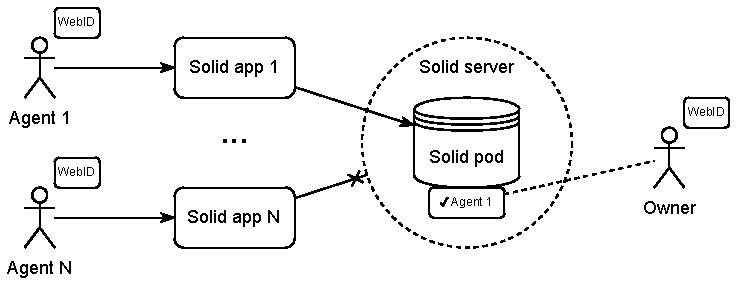
\includegraphics[width=0.62\linewidth]{./img/poster/concept-of-decentralization.pdf}
\end{center}
\end{posterbox}

\begin{posterbox}[column=0, name=data, below=foundations]{Data sources}
Combine sources of semi-structured and structured geodata.

\begin{enumerate}
\item OpenStreetMap dataset, Taginfo and Overpass API.
\item Wikidata and DBPedia accessed via SPARQL endpoints.
\end{enumerate}
\end{posterbox}

\begin{posterbox}[column=0, name=architecture, below=data]{Architecture}
The application follows the \emph{three-tier} architectural pattern.

\begin{center}
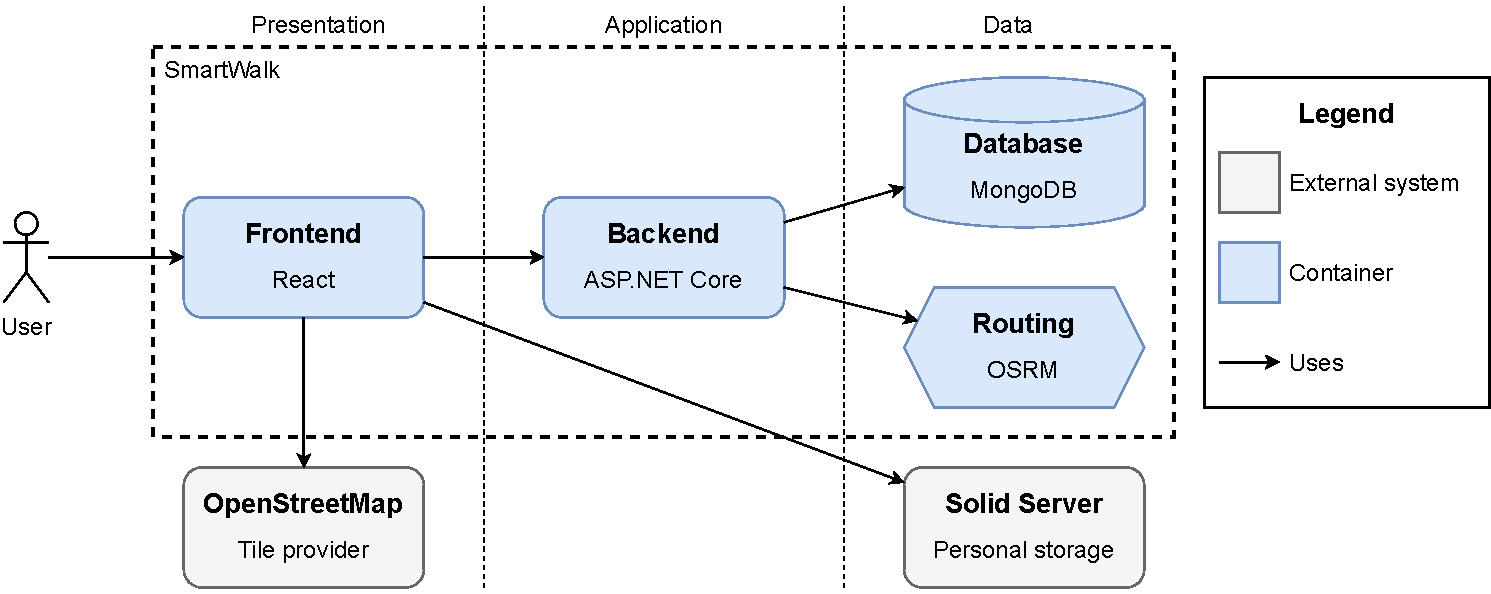
\includegraphics[width=0.98\linewidth]{./img/poster/c4-container-diagram.pdf}
\end{center}

\begin{itemize}
\item The frontend and backend communicate over HTTP.
\item The backend is stateless. Geographic entities are read-only and stored in a horizontally scalable database.
\item The backend \textbf{does not} have access to user data.
\item A specialized routing engine calculates polylines.
\end{itemize}

\end{posterbox}

%
% RIGHT COLUMN
%

\begin{posterbox}[column=1, name=ui]{User interface}
The user interface comprises \emph{12} panels. The primary feature~is category-driven declarative \emph{route} search.

\vspace{0.5em}

\begin{minipage}{1.00\textwidth}
\begin{minipage}{0.49\textwidth}
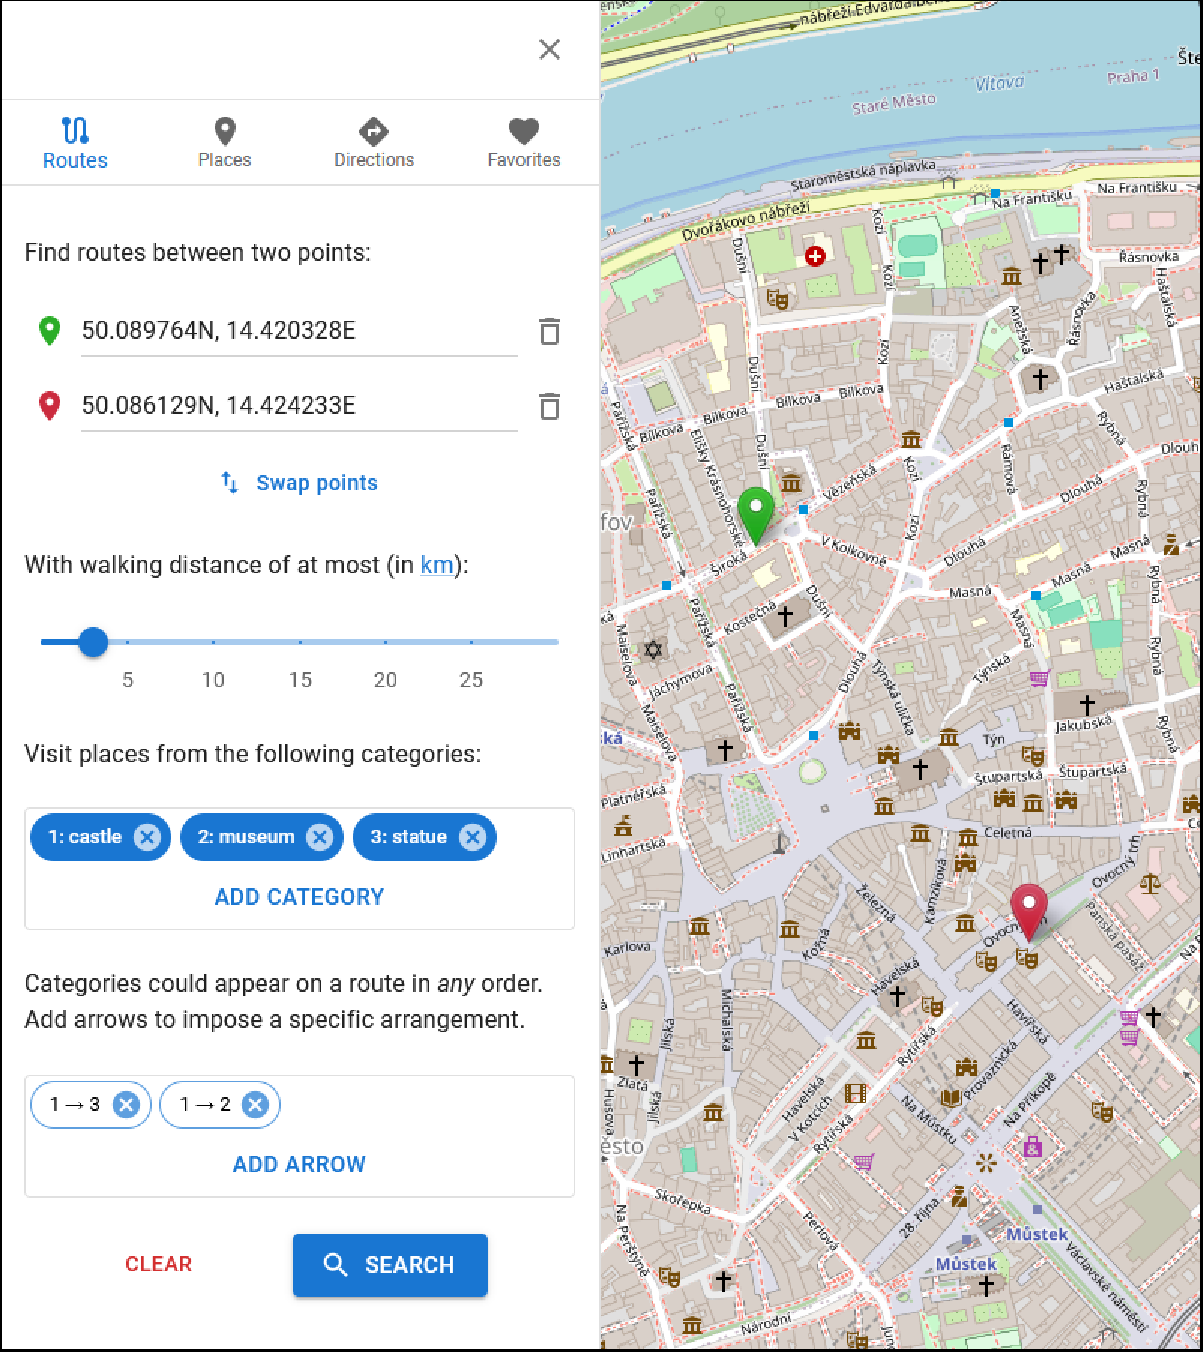
\includegraphics[width=1.00\linewidth]{./img/poster/uc04-search-routes-config.pdf}
\end{minipage}
\hfill
\begin{minipage}{0.49\textwidth}
\centering
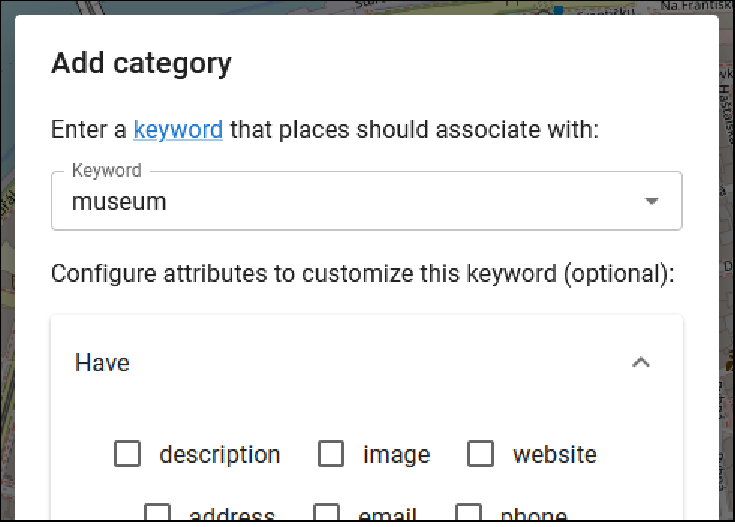
\includegraphics[width=0.65\linewidth]{./img/poster/configure-category.pdf} \\
\vspace{0.35em}
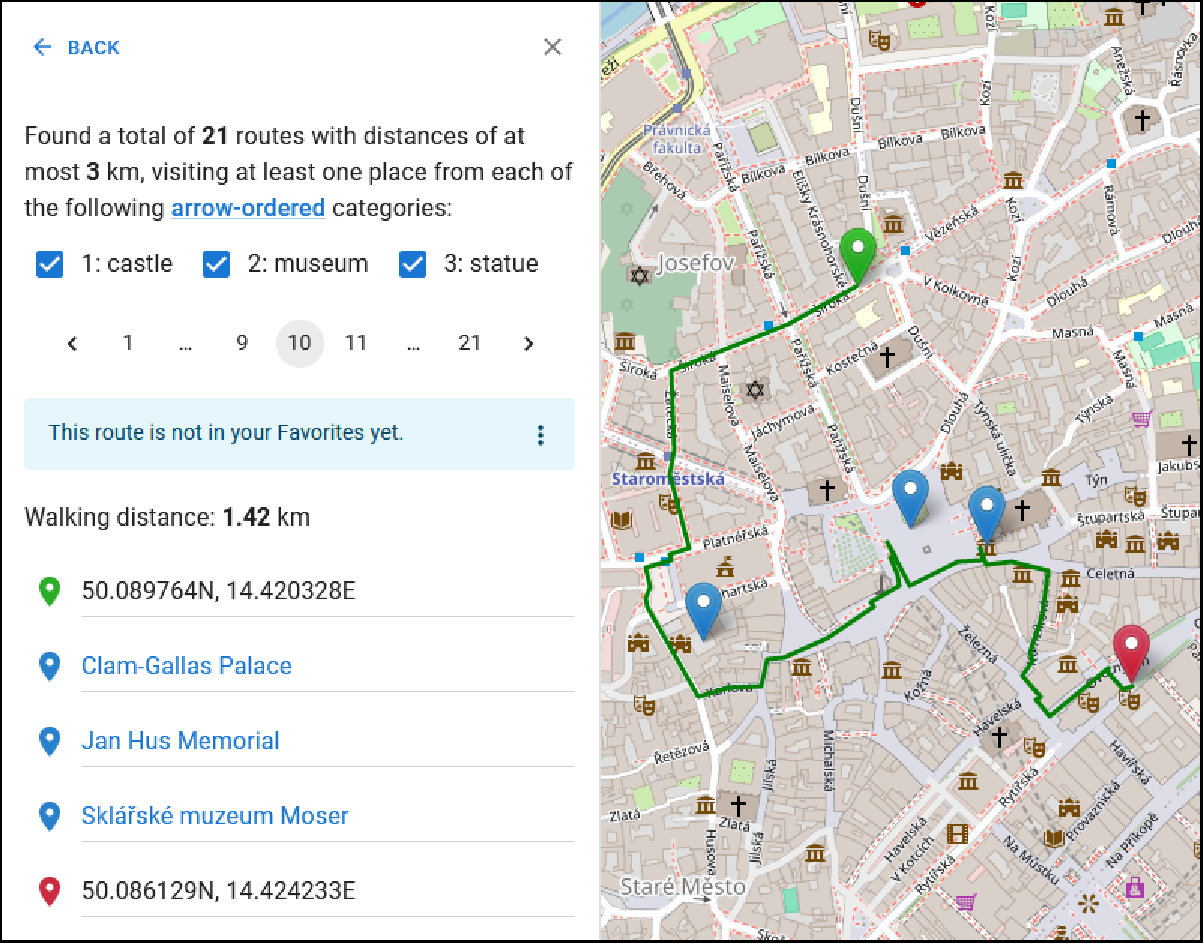
\includegraphics[width=1.00\linewidth]{./img/poster/uc04-search-routes-result.pdf}
\end{minipage}
\end{minipage}

\vspace{0.5em}

Besides routes, the application supports \emph{place} and standard location-driven \emph{direction} search. Access saved entities via the ``Favorites'' panel.

\vspace{0.5em}

\begin{minipage}{1.00\textwidth}
\begin{minipage}{0.62\textwidth}
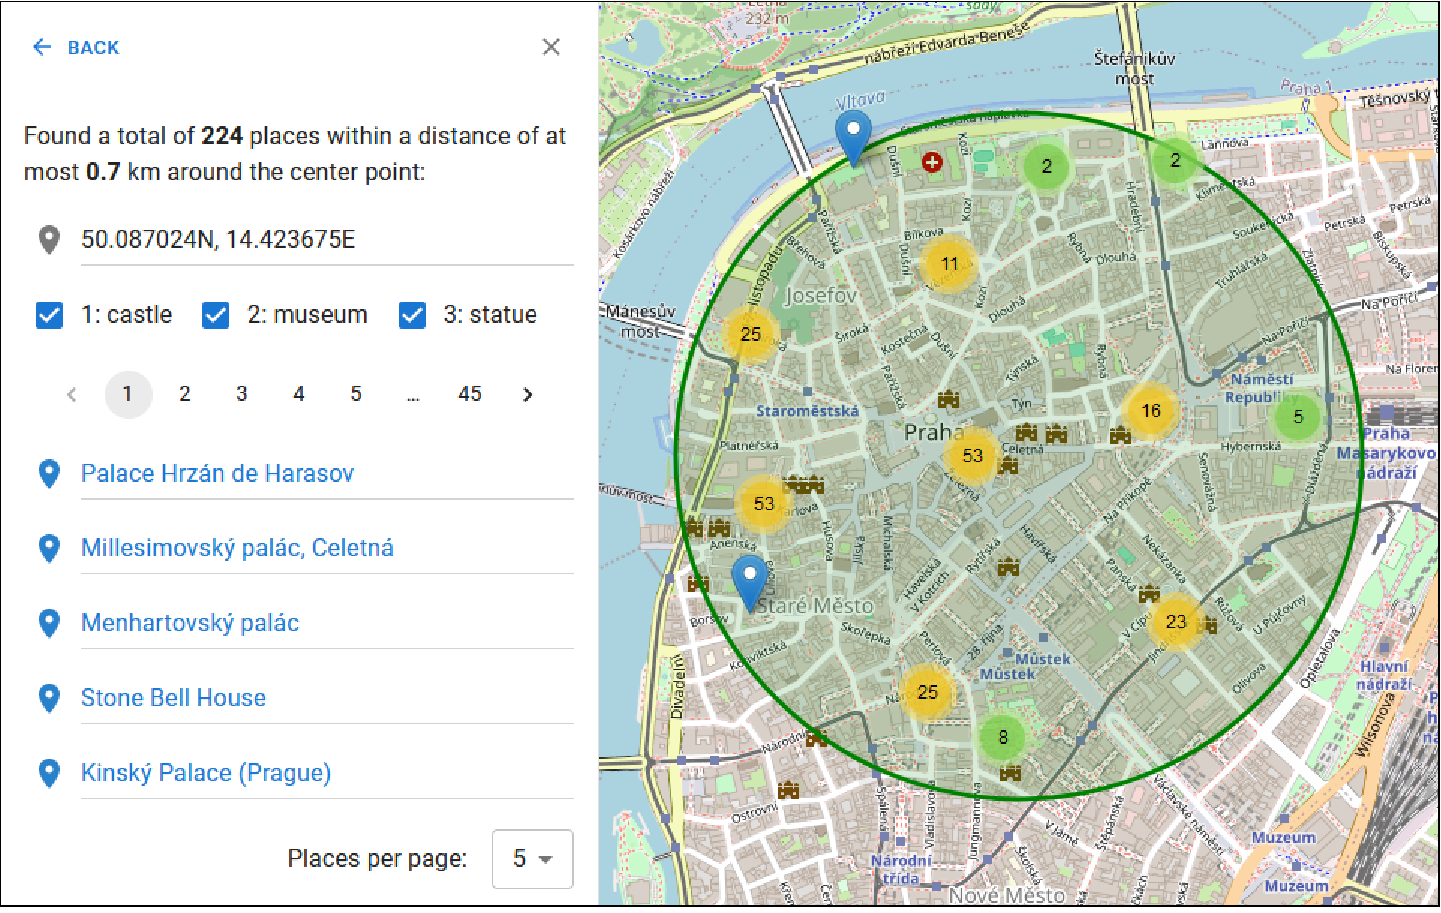
\includegraphics[width=1.00\linewidth]{./img/poster/result-places.pdf}
\end{minipage}
\hfill
\begin{minipage}{0.36\textwidth}
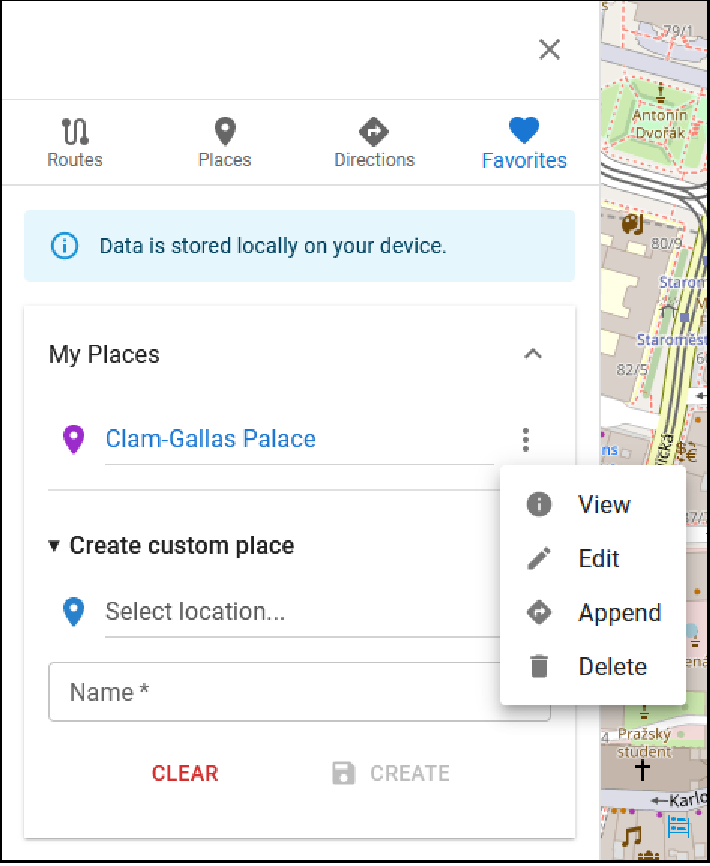
\includegraphics[width=1.00\linewidth]{./img/poster/favorites.pdf}
\end{minipage}
\end{minipage}

\vspace{0.5em}

\textbf{(!)} A user can activate a Solid pod, but it is \textbf{not} mandatory.
\end{posterbox}

\begin{posterbox}[column=1, name=results, below=ui, headerColorOne=green!50, boxColorOne=green!10]{Main results}
\begin{itemize}
\item Designed, developed, and tested a web app that fulfills all stated requirements.
\item Queries $\leq$~5km take $\leq$~1s for places, and $\leq$~2s for routes. Direction search is fast, $\leq$~30ms.
\item The UI may feel cumbersome, but it is easy to learn.
\item Opensource, Docker-enabled, deployable on a laptop.
\end{itemize}
\end{posterbox}

\begin{posterbox}[column=1, name=future, below=results]{Future work}
\begin{itemize}
\item Design a richer system of metadata for stored entities.
\item Enable user collaboration through Solid pods. Use RDF.
\item Experiment with path-finding algorithms and heuristics.
\item Apply advanced data mining and keyword extraction.
\end{itemize}
\end{posterbox}

\begin{posterbox}[column=1, name=contact, below=future, bottomaligned=architecture]{Contact}
\begin{minipage}{1.00\textwidth}
\begin{minipage}{0.10\textwidth}

\includegraphics[width=1.00\linewidth]{./img/poster/qr.pdf}
\end{minipage}
\hfill
\begin{minipage}{0.885\textwidth}
zhukov.dm.s@gmail.com \\
https://github.com/zhukovdm/smartwalk
\end{minipage}
\end{minipage}
\end{posterbox}

\end{poster}
\end{document}
